\documentclass[10pt,a4paper]{article}
\usepackage[T1]{fontenc}
\usepackage[utf8]{inputenc}
\usepackage{lmodern}
\usepackage[a4paper,margin=18mm,headheight=14pt,footskip=10mm]{geometry}
\usepackage{graphicx}
\usepackage{array,tabularx,booktabs,longtable,multirow}
\usepackage{microtype}
\usepackage{enumitem}
\usepackage{xcolor}
\usepackage{hyperref}
\usepackage{fancyhdr}
\usepackage{pdflscape}
\usepackage{float}
\usepackage{caption}
\usepackage{needspace}
\usepackage{ragged2e}
\usepackage{tikz}
\usepackage{url}
\hypersetup{colorlinks=true,linkcolor=blue!45!black,urlcolor=blue!45!black,pdftitle={BookEase Cloud Deployment - SE-490 CEA},pdfauthor={Group 19}}
\definecolor{navy}{HTML}{123455}
\definecolor{muted}{HTML}{536376}
\definecolor{lightblue}{HTML}{EAF2F9}
\definecolor{ruleblue}{HTML}{B7CADC}
\setlength{\parindent}{0pt}
\setlength{\parskip}{4pt}
\setlist[itemize]{leftmargin=*,topsep=2pt,itemsep=1pt,parsep=0pt}
\setlist[enumerate]{leftmargin=*,topsep=2pt,itemsep=1pt,parsep=0pt}
\renewcommand{\arraystretch}{1.16}
\makeatletter
\renewcommand{\section}{\@startsection{section}{1}{0pt}{11pt}{5pt}{\normalfont\large\bfseries\color{navy}}}
\renewcommand{\subsection}{\@startsection{subsection}{2}{0pt}{7pt}{3pt}{\normalfont\normalsize\bfseries\color{navy}}}
\makeatother
\pagestyle{fancy}
\fancyhf{}
\lhead{\small\textcolor{muted}{BookEase Cloud Deployment | SE-490 CEA}}
\rhead{\small\textcolor{muted}{Group 19}}
\cfoot{\small\thepage}
\renewcommand{\headrulewidth}{0.4pt}
\setlength{\emergencystretch}{2em}
\newcommand{\service}[1]{\textbf{#1}}
\newcommand{\tagline}[1]{\vspace{1mm}\textcolor{muted}{\small #1}}
\newcommand{\evidence}[3]{%
\begin{center}
  {\bfseries\small #1}\par\vspace{3pt}
  \IfFileExists{screenshots/#2}{%
    \includegraphics[width=0.94\linewidth,height=72mm,keepaspectratio]{screenshots/#2}%
  }{%
    \fcolorbox{ruleblue}{lightblue}{%
      \parbox[c][68mm][c]{0.88\linewidth}{%
        \centering\sffamily\small SCREENSHOT PLACEHOLDER\\[5pt]
        \textbf{#1}\\[7pt]
        \scriptsize\texttt{#2}\\[5pt]
        \scriptsize Place the image in the \texttt{screenshots/} folder}%
    }%
  }\par\vspace{2pt}
  {\footnotesize\color{muted}#3}\par
\end{center}
}
\begin{document}

% ------------ COVER / TITLE PAGE ------------
\thispagestyle{empty}
\vspace*{16mm}
\begin{center}
{\Large\bfseries NED UNIVERSITY OF ENGINEERING \& TECHNOLOGY -- 75270,\\[2pt] KARACHI}\par
\vspace{7mm}
{\large\bfseries DEPARTMENT OF SOFTWARE ENGINEERING}\par
\vspace{21mm}
{\Large\bfseries Cloud Computing (SE-490)}\par
\vspace{4mm}
{\Large\bfseries Complex Engineering Activity (CEA)}\par
\vspace{15mm}
{\color{navy}\Huge\bfseries BookEase Cloud Deployment}\par
\vspace{7mm}
{\large\bfseries Design, Deployment, and Cloud-Native Enhancement\\[3pt] of a Three-Tier Web Application}\par
\vspace{16mm}
{\Large\bfseries Group 19}\par
\vspace{8mm}
\begin{tabular}{>{\raggedright\arraybackslash}p{70mm} >{\centering\arraybackslash}p{35mm}}
\toprule
\textbf{Group members} & \textbf{Roll number}\\
\midrule
Muhammad Abdullah Khan & SE-23061\\
Muhammad Rafay & SE-23100\\
\bottomrule
\end{tabular}
\par\vspace{9mm}
{\large\bfseries Section B}\par
\vspace{7mm}
\begin{tabular}{rl}
\textbf{SEMESTER:} & 7th (FALL 2026)\\
\textbf{INSTRUCTOR:} & Engr. Aminah Akhtar\\
\textbf{Submission Date:} & 10th November 2026\\
\end{tabular}
\end{center}
\vfill
\begin{center}\small Department of Software Engineering \textbullet\ Karachi, Pakistan\end{center}
\clearpage

% ------------ ARCHITECTURE DIAGRAM ------------
\begin{landscape}
\thispagestyle{plain}
\begin{center}
{\LARGE\bfseries\color{navy}1. Architecture Diagram}\par\vspace{3mm}
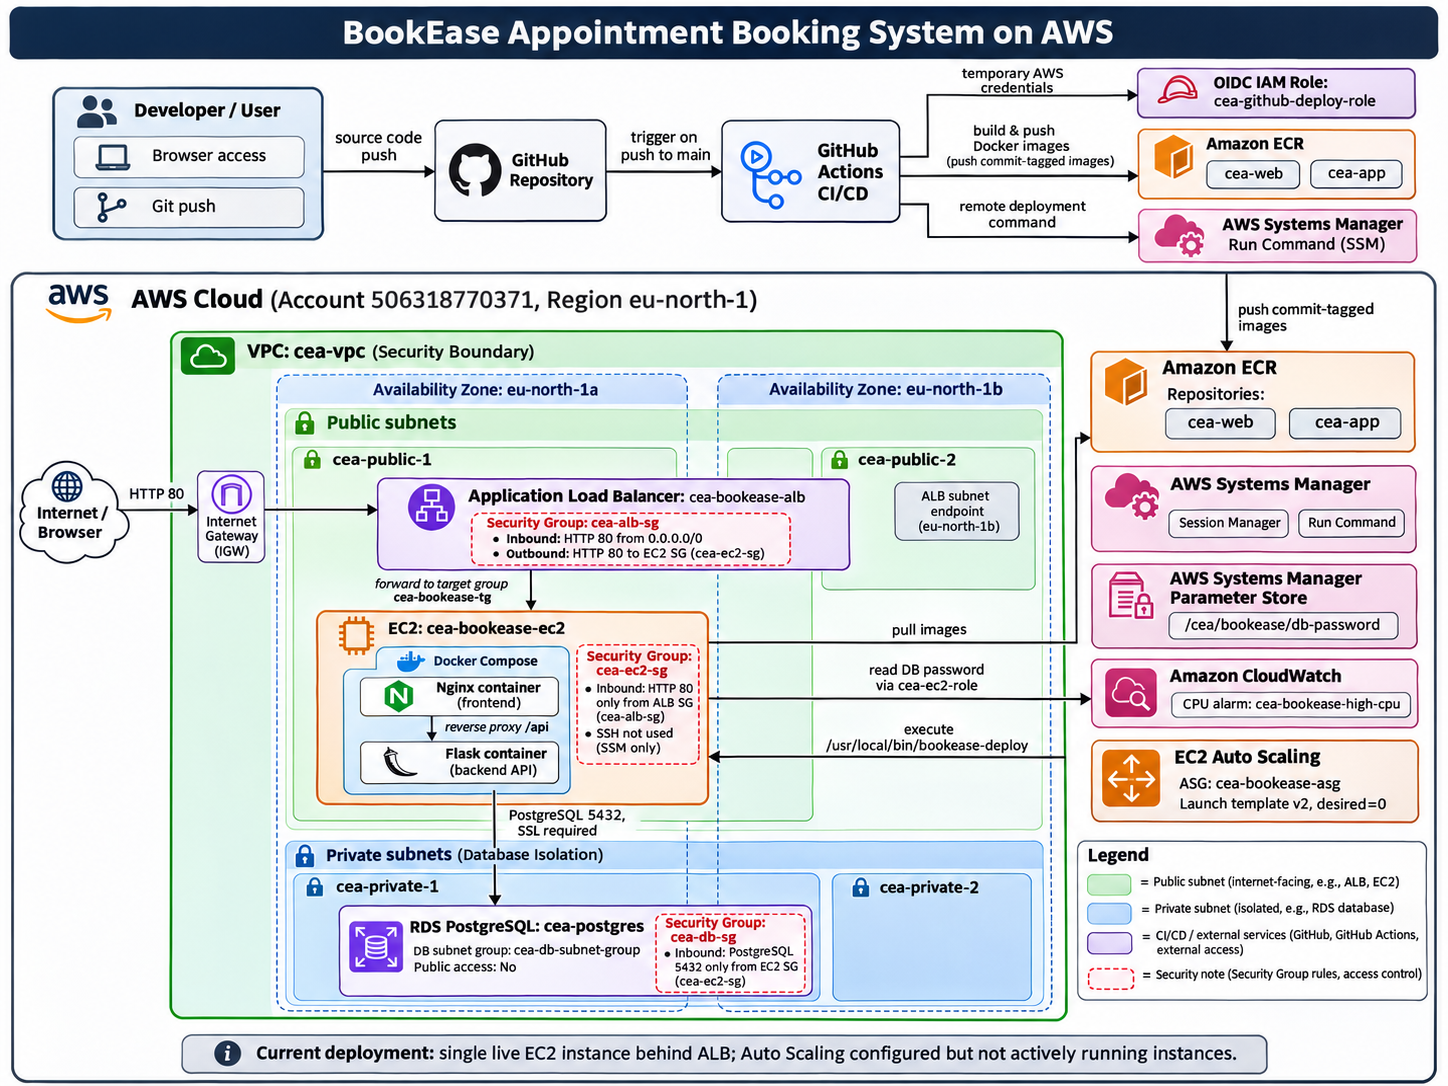
\includegraphics[width=0.97\linewidth,height=0.86\textheight,keepaspectratio]{figures/bookease-architecture.png}
\par\vspace{2mm}
{\footnotesize\color{muted}Figure 1. Network segmentation, three tiers, ALB routing, container registry, OIDC CI/CD, secrets, management and monitoring. Diagram is conceptual: the deployed Single-AZ RDS instance is in eu-north-1b; the DB subnet group spans both private subnets. ASG desired capacity is 0.}
\end{center}
\end{landscape}
\clearpage

% ------------ REPORT PAGE 1 ------------
\section*{2. Technical Report (Page 1 of 5): Project Overview and Design}
\subsection*{2.1 Objective and cloud provider selection}
\textbf{BookEase} is a three-tier appointment booking web application built for the SE-490 Complex Engineering Activity. Users can view appointment slots, create reservations and inspect saved bookings. Its web presentation, application logic and persistent data are separated logically and deployed on Amazon Web Services (AWS), region \texttt{eu-north-1} (Stockholm). The resulting system was accessed through the public Application Load Balancer (ALB) and was validated with actual PostgreSQL-backed bookings.

AWS was selected because its integrated VPC networking, EC2 compute, managed RDS, private Elastic Container Registry (ECR), IAM/OIDC, Systems Manager and CloudWatch match the assignment's infrastructure, security and CI/CD requirements. Managed services reduce database administration, while established APIs and the GitHub Actions ecosystem support repeatable deployment. Small-instance sizing and use of existing AWS credits were considered for coursework cost control, but running resources can still incur charges.

\subsection*{2.2 Three-tier architecture}
\begin{tabularx}{\linewidth}{@{}p{21mm}p{35mm}X@{}}
\toprule
\textbf{Tier} & \textbf{Implementation} & \textbf{Responsibility / connectivity}\\
\midrule
Web & Nginx Docker image \texttt{cea-web} & Serves HTML/CSS/JavaScript and reverse-proxies \texttt{/api/} to the application service by Docker DNS name \texttt{app:5000}. Only HTTP port 80 is published on EC2.\\
Application & Flask + Gunicorn Docker image \texttt{cea-app} & Validates bookings, reads appointment availability, creates/deletes records and accesses PostgreSQL through \texttt{DATABASE\_URL}. Port 5000 is internal to the Docker bridge network.\\
Database & Amazon RDS PostgreSQL \texttt{cea-postgres} & Durable \texttt{appointmentdb} storage; private DB subnet group, no public access, TCP 5432 limited to the EC2 security group.\\
\bottomrule
\end{tabularx}

\subsection*{2.3 VPC, availability zones and routing}
The custom \texttt{cea-vpc} uses \texttt{10.0.0.0/16}. Four /24 subnets are distributed across two Availability Zones. The ALB occupies two public subnets for multi-zone ingress; the currently deployed application containers share one EC2 host in \texttt{cea-public-1}. The private subnet group supports RDS placement; the active RDS instance is Single-AZ in \texttt{eu-north-1b}.

\begin{tabularx}{\linewidth}{@{}p{30mm}p{28mm}p{28mm}X@{}}
\toprule
\textbf{Subnet} & \textbf{CIDR} & \textbf{AZ} & \textbf{Purpose}\\
\midrule
\texttt{cea-public-1} & \texttt{10.0.1.0/24} & eu-north-1a & ALB and primary EC2 host\\
\texttt{cea-public-2} & \texttt{10.0.2.0/24} & eu-north-1b & ALB second-zone subnet\\
\texttt{cea-private-1} & \texttt{10.0.3.0/24} & eu-north-1a & RDS subnet-group member\\
\texttt{cea-private-2} & \texttt{10.0.4.0/24} & eu-north-1b & RDS subnet-group member / active DB AZ\\
\bottomrule
\end{tabularx}

The public route table directs \texttt{0.0.0.0/0} to \texttt{cea-igw}; the private route table retains only VPC-local routing. A NAT gateway was not provisioned because the isolated RDS database does not require outbound internet access. ALB traffic is forwarded to the \texttt{cea-bookease-tg} instance target group on HTTP 80 with health-check path \texttt{/api/health}. These choices provide public entry at the ALB while keeping database network access private.
\clearpage

% ------------ REPORT PAGE 2 ------------
\section*{2. Technical Report (Page 2 of 5): Services and Security}
\subsection*{2.4 AWS services and deployed roles}
\begin{tabularx}{\linewidth}{@{}p{35mm}X@{}}
\toprule
\textbf{Service / resource} & \textbf{Role in BookEase}\\
\midrule
EC2 \texttt{cea-bookease-ec2} & Amazon Linux 2023 x86\_64, \texttt{t3.micro}; Docker Engine and Compose run the web and application containers.\\
ALB \texttt{cea-bookease-alb} & Internet-facing HTTP listener, traffic forwarding and registered-target health monitoring.\\
RDS \texttt{cea-postgres} & Managed PostgreSQL, \texttt{appointmentdb}, Single-AZ, private access, 20 GiB storage.\\
Amazon ECR & Private immutable repositories \texttt{cea-web} and \texttt{cea-app}; \texttt{v1} and Git-SHA image tags.\\
AWS Systems Manager & Session Manager for administration without SSH; Run Command for CI/CD deployment and Parameter Store for a protected DB password.\\
IAM & EC2 instance profile \texttt{cea-ec2-role}; OIDC deployment role \texttt{cea-github-deploy-role}.\\
CloudWatch & \texttt{cea-bookease-high-cpu} alarm: average CPU utilization greater than 70\% for two five-minute datapoints.\\
EC2 Auto Scaling & \texttt{cea-bookease-asg}, launch-template version 2, capacity min/desired/max = 0/0/2; configuration prepared, not active scale-out.\\
\bottomrule
\end{tabularx}

\subsection*{2.5 Security boundaries and secret handling}
\begin{tabularx}{\linewidth}{@{}p{29mm}p{36mm}X@{}}
\toprule
\textbf{Security group} & \textbf{Inbound rule} & \textbf{Rationale}\\
\midrule
\texttt{cea-alb-sg} & TCP 80 from \texttt{0.0.0.0/0} & Public traffic terminates at the load balancer; ALB outbound HTTP reaches the EC2 SG.\\
\texttt{cea-ec2-sg} & TCP 80 from \texttt{cea-alb-sg} & Direct internet access to the app host is blocked at ingress; port 5000 is not published.\\
\texttt{cea-db-sg} & TCP 5432 from \texttt{cea-ec2-sg} & PostgreSQL accepts connections only from the application host security group.\\
\bottomrule
\end{tabularx}

The database has \textbf{Public access = No}. Administration uses SSM Session Manager instead of inbound SSH. The RDS password resides in a Parameter Store \texttt{SecureString} at \texttt{/cea/bookease/db-password}; an IAM inline policy permits the EC2 role to read only this parameter. EC2 generates root-readable \texttt{/opt/bookease/backend.env} (mode \texttt{0600}) without putting credentials in GitHub or ECR. The PostgreSQL URL specifies \texttt{sslmode=require}, encrypting the database connection. More stringent certificate verification (\texttt{verify-full}) is a recommended improvement.

GitHub Actions assumes an IAM role using GitHub's OIDC provider and a trust condition restricted to the intended repository and \texttt{main} branch. It receives temporary credentials rather than root keys; ECR permissions are scoped to the two repositories and SSM Run Command to the designated EC2 instance. The operational limitation is that an SSM shell command still has powerful access to that instance; branch protection, audited approvals and separate deployment roles would strengthen production controls.

\textbf{Known exposure:} The ALB currently serves HTTP, not HTTPS. Testing used fictional contact data; production handling of real personal information requires an ACM-backed HTTPS listener, HTTP-to-HTTPS redirect and stricter secret management.
\clearpage

% ------------ REPORT PAGE 3 ------------
\section*{2. Technical Report (Page 3 of 5): Containers, CI/CD and Sources}
\subsection*{2.6 Container build and local orchestration}
Separate Dockerfiles define the two tiers: \texttt{frontend/Dockerfile} creates an Nginx image and copies the web assets and reverse-proxy configuration; \texttt{backend/Dockerfile} packages the Flask API and dependencies, launches Gunicorn and runs as a non-root application user. The local \texttt{docker-compose.yml} combines the web and application containers; a local PostgreSQL container was used during development. Production replaces that local database with managed RDS. On EC2, \texttt{/opt/bookease/compose.yaml} references ECR images and mounts the protected DB environment file into the application service.

The public path is \textbf{Browser $\rightarrow$ ALB:80 $\rightarrow$ Nginx:80 $\rightarrow$ Flask:5000 $\rightarrow$ RDS:5432}. This is a logical three-tier design; the web and application tiers are on the \emph{same public-subnet EC2 host} and separated by a private Docker bridge, not by distinct EC2 private subnets. This is a coursework trade-off rather than full physical network isolation of the application tier.

\subsection*{2.7 Automated build, registry and deployment}
GitHub Actions is defined in \texttt{.github/workflows/deploy.yml}. Pushing to \texttt{main} triggers the pipeline automatically (\texttt{workflow\_dispatch} also allows manual runs). Its stages are:
\begin{enumerate}
\item Checkout source; set up Python 3.12; install backend requirements; compile Python and run Flask health-endpoint unit tests.
\item Assume \texttt{cea-github-deploy-role} via OIDC; authenticate Docker to ECR with temporary AWS credentials.
\item Build and push \texttt{cea-web} and \texttt{cea-app}, tagged with the full \texttt{github.sha} commit identifier; immutable tags support traceability.
\item Invoke SSM Run Command on the designated EC2 instance to execute \texttt{/usr/local/bin/bookease-deploy} with the commit SHA.
\item The deployment script pulls both images before replacing containers, updates \texttt{BOOKEASE\_TAG} in Docker Compose and tests \texttt{/api/appointments}. Pipeline status fails if the deployed service does not pass the check.
\end{enumerate}

Two observed successful workflow runs correspond to commits \texttt{ea36fc5} and \texttt{abd82dc}. EC2's \texttt{docker ps} output subsequently showed \emph{both} Nginx and Flask images tagged \texttt{abd82dcf47ac3f2c3004b923d50ef6c046888a8c}, demonstrating release traceability from GitHub to running containers.

\subsection*{2.8 Source deliverables and repository}
\small
\begin{tabularx}{\linewidth}{@{}p{57mm}X@{}}
\toprule
\textbf{Source artifact} & \textbf{Location / purpose}\\
\midrule
Frontend Dockerfile / Nginx config & \texttt{frontend/Dockerfile}; \texttt{frontend/nginx.conf}\\
Backend Dockerfile / Flask source & \texttt{backend/Dockerfile}; \texttt{backend/app.py}; \texttt{backend/database.py}\\
Local multi-container definition & \texttt{docker-compose.yml}\\
Production Compose and deployment & \texttt{/opt/bookease/compose.yaml}; EC2 \texttt{/usr/local/bin/bookease-deploy} (server-side files)\\
GitHub Actions pipeline & \texttt{.github/workflows/deploy.yml}\\
Automated health test & \texttt{backend/tests/test\_health\_ci.py}\\
Auto Scaling bootstrap & \texttt{infrastructure/asg-user-data.sh}; launch template v2\\
Kubernetes manifests & Not applicable: Docker Compose on EC2, not Kubernetes\\
\bottomrule
\end{tabularx}
\normalsize
\textbf{Repository:} \url{https://github.com/rafay-2003/appointment-booking-cea}. Protected \texttt{.env} files and cloud database credentials are excluded from source control. The server-side Compose/deployment script should also be archived in the submitted source bundle if required by the instructor.
\clearpage

% ------------ REPORT PAGE 4 ------------
\section*{2. Technical Report (Page 4 of 5): Verification and Observations}
\subsection*{2.9 Deployment validation and functional testing}
\begin{tabularx}{\linewidth}{@{}p{51mm}p{22mm}X@{}}
\toprule
\textbf{Test / observation} & \textbf{Outcome} & \textbf{Evidence and interpretation}\\
\midrule
Docker startup on EC2 & Passed & \texttt{cea-nginx-web} and \texttt{cea-flask-app} reported \texttt{Up}.\\
Local health route & Passed & \texttt{GET /api/health} through Nginx responded HTTP 200.\\
RDS-backed appointment listing & Passed & After one-time \texttt{initialize\_database()}, \texttt{GET /api/appointments} returned HTTP 200.\\
Appointment insertion & Passed & Test booking \texttt{CEA Test User}, 2026-11-12, 10:00 was stored with record ID 1 and returned by GET.\\
Booked-slot validation & Passed & \texttt{GET /api/slots?date=2026-11-12} reported \texttt{booked\_slots:["10:00"]}.\\
ALB routing and target health & Passed & \texttt{cea-bookease-tg} target reported Healthy with check \texttt{/api/health}.\\
Browser end-to-end interaction & Passed & BookEase loaded via public ALB DNS; a second booking persisted after browser refresh.\\
Automated CI/CD & Passed & GitHub Actions runs \#1 and \#2 successful; EC2 containers showed matching \texttt{abd82dc...} commit tags.\\
CloudWatch metric visibility & Observed & CPU graph showed datapoints and a 70\% alarm threshold; an alarm firing was not tested.\\
ASG horizontal scaling & Not tested & Launch template v2, ASG and CPU policy configured, but desired capacity remained 0; not attached to live ALB.\\
\bottomrule
\end{tabularx}

\subsection*{2.10 Debugging record}
During deployment, \texttt{/api/appointments} initially returned HTTP 500 despite the health endpoint being healthy. Flask logs revealed \texttt{psycopg.errors.UndefinedTable}: the new RDS database lacked the \texttt{appointments} table used during local development. Running the existing backend \texttt{initialize\_database()} function created the schema. Both the appointment and slot endpoints then returned HTTP 200; a stored booking subsequently demonstrated successful reads and writes. This incident illustrates why health endpoints alone do not prove database readiness.

\subsection*{2.11 Scope of demonstrated automation and known limits}
The observed deployment automated a new version on \textbf{one existing EC2 instance}. The current deployment script is intentionally tied to that instance's ID and is not an ASG-wide rolling updater. A new ASG instance would depend on launch-time user data and a fixed image SHA; its successful bootstrapping has not been observed. The project therefore demonstrates automated single-host delivery plus an \emph{ASG configuration}, not fault-tolerant multi-instance production deployment.

Other limitations include a single EC2 host, a Single-AZ database, no real load or failover test, HTTP-only public ingress, no automatic DB credential rotation, and possible brief downtime when Docker Compose recreates containers. These are important constraints on availability, elasticity and security claims.
\clearpage

% ------------ REPORT PAGE 5 ------------
\section*{2. Technical Report (Page 5 of 5): NFR Justification}
\subsection*{2.12 Requirement 10 --- mapping quality attributes to implementation}
\footnotesize
\begin{tabularx}{\linewidth}{@{}p{27mm}p{68mm}X@{}}
\toprule
\textbf{NFR} & \textbf{Design / implementation justification} & \textbf{Limitation / improvement}\\
\midrule
\textbf{Scalability} & Stateless Flask/Gunicorn instances can be built identically from ECR images; ALB target groups and a 0--2-instance ASG configuration provide a horizontal scaling path. & ASG desired=0, no registered ASG targets. Bootstrap and shared rollout must be verified before claiming real scale-out.\\
\textbf{Availability / Reliability} & ALB spans two public subnets/AZs and probes \texttt{/api/health}; managed RDS and Docker restart policies improve recoverability. & Only one live EC2 and Single-AZ RDS are used. Add at least two ASG instances and Multi-AZ RDS for resilience.\\
\textbf{Elasticity} & Target-tracking scaling policy configured at 60\% average CPU with 300 s warmup; launch template includes bootstrap user data. & At desired=0 the group has no instances producing CPU metrics, so scaling cannot yet be demonstrated. Activate/test ASG and add a minimum running capacity.\\
\textbf{Security} & VPC public/private segmentation, ALB/EC2/RDS SG chaining, database no-public-access, SSM instead of SSH, OIDC with scoped IAM, Parameter Store SecureString and RDS TLS required. & Public ingress is HTTP only; TLS certificate validation is not strict. Add HTTPS/ACM, verify-full, approval gates and secret rotation.\\
\textbf{Maintainability / Deployability} & Separate Dockerfiles, Compose, health unit test, immutable Git-SHA ECR tags and GitHub Actions OIDC build/push/deploy reduce manual release steps. & Deployment currently targets one EC2; use ASG instance refresh/rolling deployment and automatic rollback.\\
\textbf{Performance / Latency} & Nginx serves static assets and proxies API locally on the Docker network; EC2-to-RDS traffic stays inside the same VPC/region. & No load-test measurements; \texttt{t3.micro} RAM/CPU are limited. Benchmark, monitor latency and tune Gunicorn/instance size.\\
\textbf{Cost-Efficiency} & Small \texttt{t3.micro}, Single-AZ \texttt{db.t4g.micro}, 20 GiB RDS storage, no NAT gateway, and ASG desired=0 minimize demonstration cost. & ALB, public IPv4, EBS and RDS still consume credits/charges; stop idle compute and set billing alerts.\\
\textbf{Portability} & Nginx/Flask/PostgreSQL are standard components, Dockerfiles and Compose are provider-agnostic, and application configuration is injected by environment variable. & ECR, IAM, SSM, RDS and ALB are AWS-specific; replace integrations/configuration for a cross-cloud migration.\\
\bottomrule
\end{tabularx}
\normalsize

\subsection*{2.13 Assessment and next improvements}
The validated application fulfills the core three-tier browser-to-database path and the automated GitHub-to-ECR-to-EC2 pipeline. Networking, registry, load balancer, managed database, role-based secret access and CloudWatch monitoring are implemented. Priority production upgrades are (1) ACM-backed HTTPS with HTTP redirect, (2) verified ASG bootstrap and ALB integration with CI/CD coordinated across replicas, (3) Multi-AZ RDS and a second healthy compute target, and (4) automated rollback, log aggregation and load/failover testing. The report deliberately differentiates \emph{configured} controls from \emph{tested} capabilities.
\clearpage

% ------------ DEPLOYMENT EVIDENCE: SINGLE-COLUMN FIGURES ------------
\section*{3. Deployment Evidence --- Screenshot Gallery}
\small Place screenshots into \texttt{screenshots/} using the exact filenames below. Each image will replace its placeholder automatically. All screenshots appear one after another at full-column width, never side by side.
\normalsize
\noindent\evidence{VPC configuration}{02-vpc-created.png}{Custom VPC cea-vpc, CIDR 10.0.0.0/16.}
\vspace{3mm}
\noindent\evidence{Public and private subnets}{03-four-subnets.png}{Two public and two private subnets across eu-north-1a and eu-north-1b.}
\clearpage
\section*{3. Deployment Evidence --- Continued}
\noindent\evidence{Public routing and Internet Gateway}{04b-public-routes.png}{Public route table with default route to the Internet Gateway.}
\vspace{3mm}
\noindent\evidence{ALB security group}{05a-alb-security-group.png}{Public HTTP 80 access to cea-alb-sg.}
\clearpage
\section*{3. Deployment Evidence --- Continued}
\noindent\evidence{EC2 security group}{05b-ec2-security-group.png}{HTTP 80 accepted only from cea-alb-sg.}
\vspace{3mm}
\noindent\evidence{Database security group}{05c-database-security-group.png}{PostgreSQL 5432 accepted only from cea-ec2-sg.}
\clearpage
\section*{3. Deployment Evidence --- Continued}
\noindent\evidence{Private RDS PostgreSQL instance}{06d-rds-available.png}{cea-postgres available in private network; no public database access.}
\vspace{3mm}
\noindent\evidence{ECR application image listing}{08-ecr-app.png}{Private cea-app repository with pushed v1 image and image digest.}
\clearpage
\section*{3. Deployment Evidence --- Continued}
\noindent\evidence{EC2 host and running Docker containers}{09b-ec2-docker-running.png}{Nginx and Flask containers running on cea-bookease-ec2.}
\vspace{3mm}
\noindent\evidence{Application Load Balancer target health}{10-alb-healthy-target.png}{The ALB target group reports the registered EC2 instance as Healthy.}
\clearpage
\section*{3. Deployment Evidence --- Continued}
\noindent\evidence{Successful GitHub Actions CI/CD}{11-github-actions-success.png}{Successful automated test, ECR push and SSM deployment job (add your screenshot).}
\vspace{3mm}
\noindent\evidence{Running BookEase web application}{10-bookease-public-app.png}{Browser access to BookEase through the ALB DNS and saved bookings (add your screenshot).}
\clearpage
\section*{3. Deployment Evidence --- Continued}
\noindent\evidence{RDS-backed appointment persistence}{09c-rds-booking-test.png}{POST and GET API tests and booked-slot confirmation.}
\vspace{3mm}
\noindent\evidence{Auto Scaling Group configuration}{12-auto-scaling.png}{Prepared ASG launch template and capacity configuration; scale-out not load-tested.}
\clearpage
\section*{3. Deployment Evidence --- Continued}
\noindent\evidence{CloudWatch monitoring enhancement}{13B-cloudwatch-monitoring.png}{CloudWatch CPU utilization alarm graph and 70 percent threshold.}
\clearpage
% ------------ FINAL PAGE / WORK DISTRIBUTION ------------
\section*{4. Group Work Distribution}
\textit{Proposed equal contribution allocation for Group 19. Adjust this table to reflect the work actually performed before submission.}
\vspace{6mm}
\small\begin{tabularx}{\linewidth}{@{}p{34mm}p{21mm}X p{14mm}@{}}
\toprule
\textbf{Group member} & \textbf{Roll no.} & \textbf{Assigned work packages} & \textbf{Share}\\
\midrule
Muhammad Abdullah Khan & SE-23061 & AWS networking and VPC design; public/private subnets and route tables; security groups; RDS deployment and database isolation; ALB and target-health setup; CloudWatch monitoring and evidence review. & \textbf{50\%}\\
\addlinespace
Muhammad Rafay & SE-23100 & BookEase frontend and Flask API; Dockerfiles and Compose; ECR image packaging; EC2 application deployment and testing; GitHub Actions OIDC CI/CD; ASG launch configuration and report integration. & \textbf{50\%}\\
\bottomrule
\end{tabularx}\normalsize
\vspace{9mm}
\textbf{Joint activities:} architecture review, end-to-end verification, non-functional requirement analysis, test evidence selection, and final report proofreading.
\vfill
\begin{center}\small\textcolor{muted}{End of BookEase Cloud Deployment --- Complex Engineering Activity, Group 19}\end{center}
\end{document}
